
% % \begin{figure}[ht!]
% %     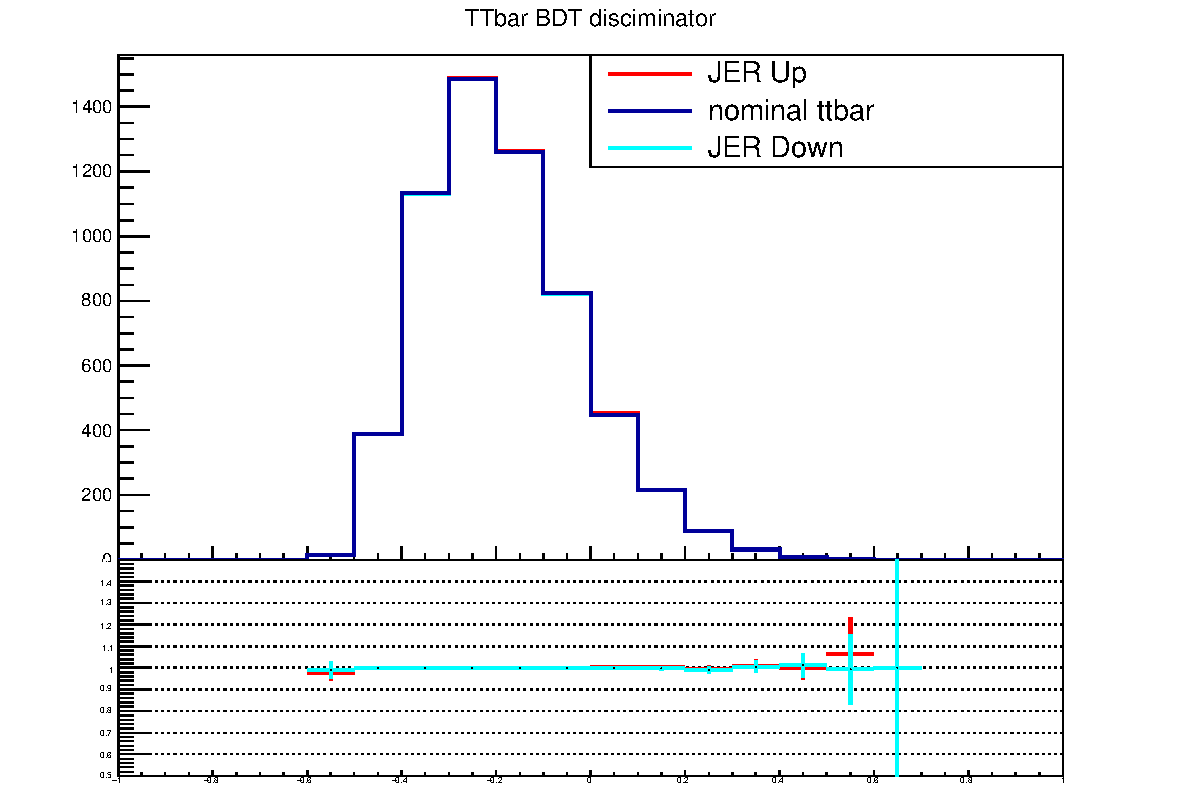
\includegraphics[width=0.48\textwidth]{images/Run2/Sys/JERsystt.pdf}
% %     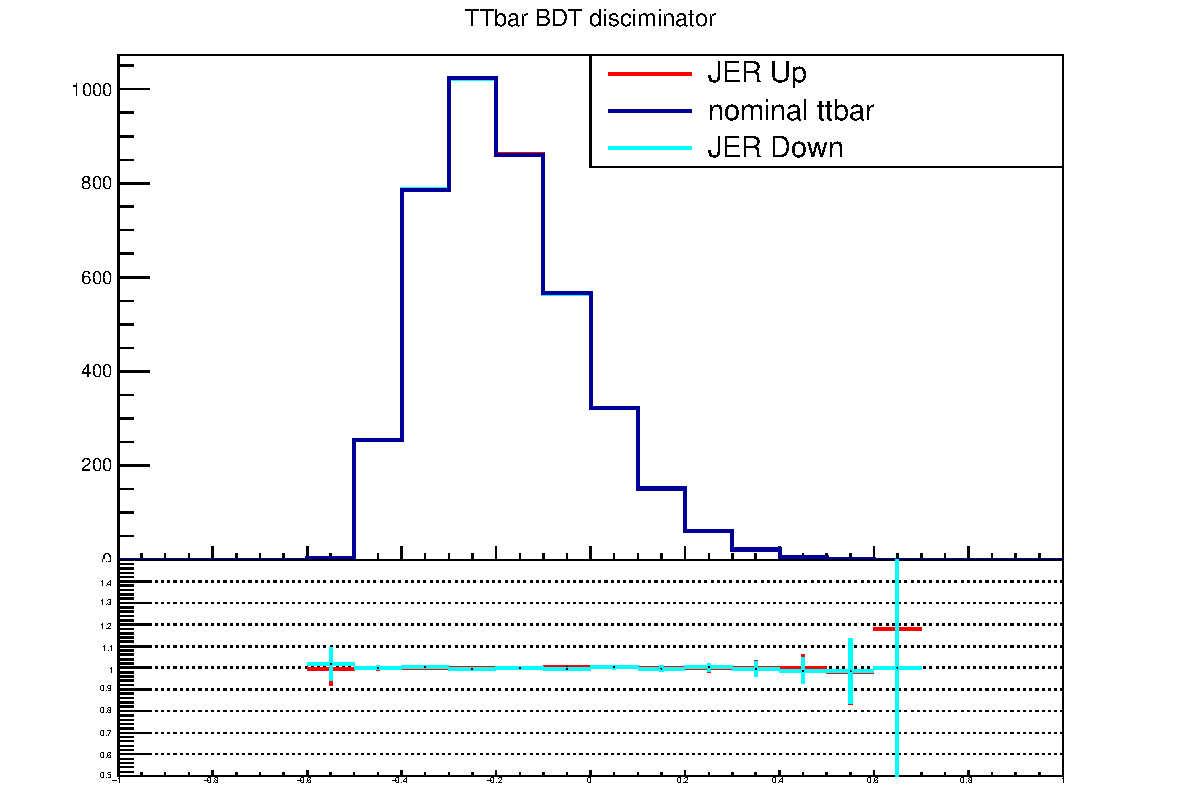
\includegraphics[width=0.48\textwidth]{images/Run2/Sys/JERsystt_e.pdf}     
% %     \caption{The BDT shapes for JER systematic in \ttbar for the $\mu$ + jets channel (left) and e + jets channel (right).}
% %     \label{fig:SysShapesJERtt}
% % \end{figure}

% % \begin{figure}[ht!]
% %     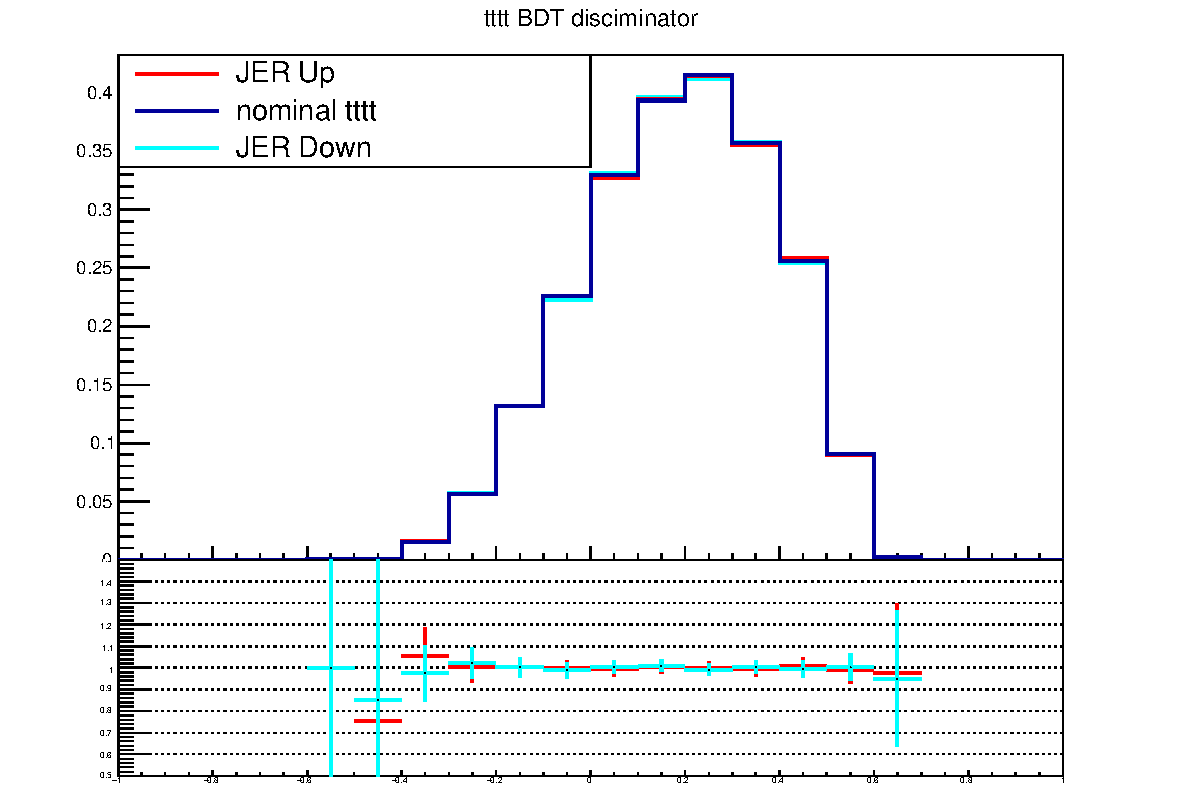
\includegraphics[width=0.48\textwidth]{images/Run2/Sys/JERsystttt.pdf}
% %     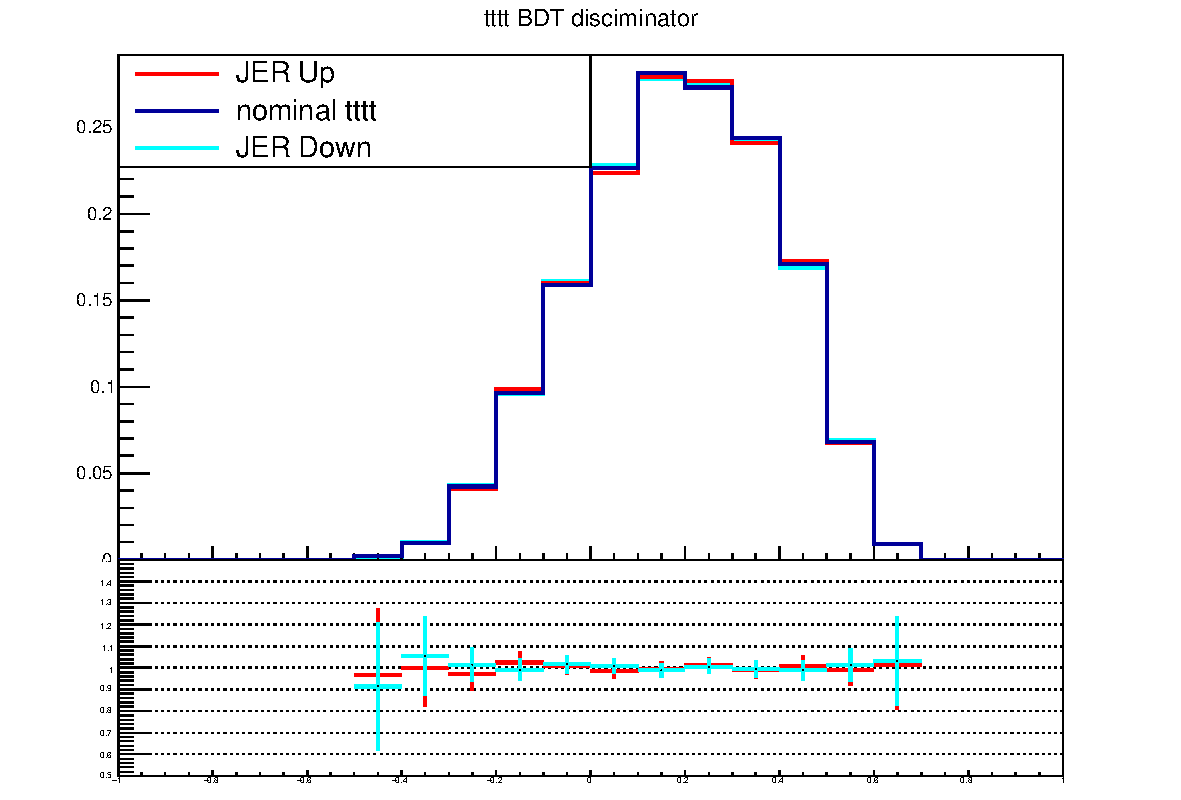
\includegraphics[width=0.48\textwidth]{images/Run2/Sys/JERsystttt_e.pdf}     
% %     \caption{The BDT shapes for JER systematic in \tttt for the $\mu$ + jets channel (left) and e + jets channel (right).}
% %     \label{fig:SysShapesJERtttt}
% % \end{figure}

% \begin{figure}[ht!]
%     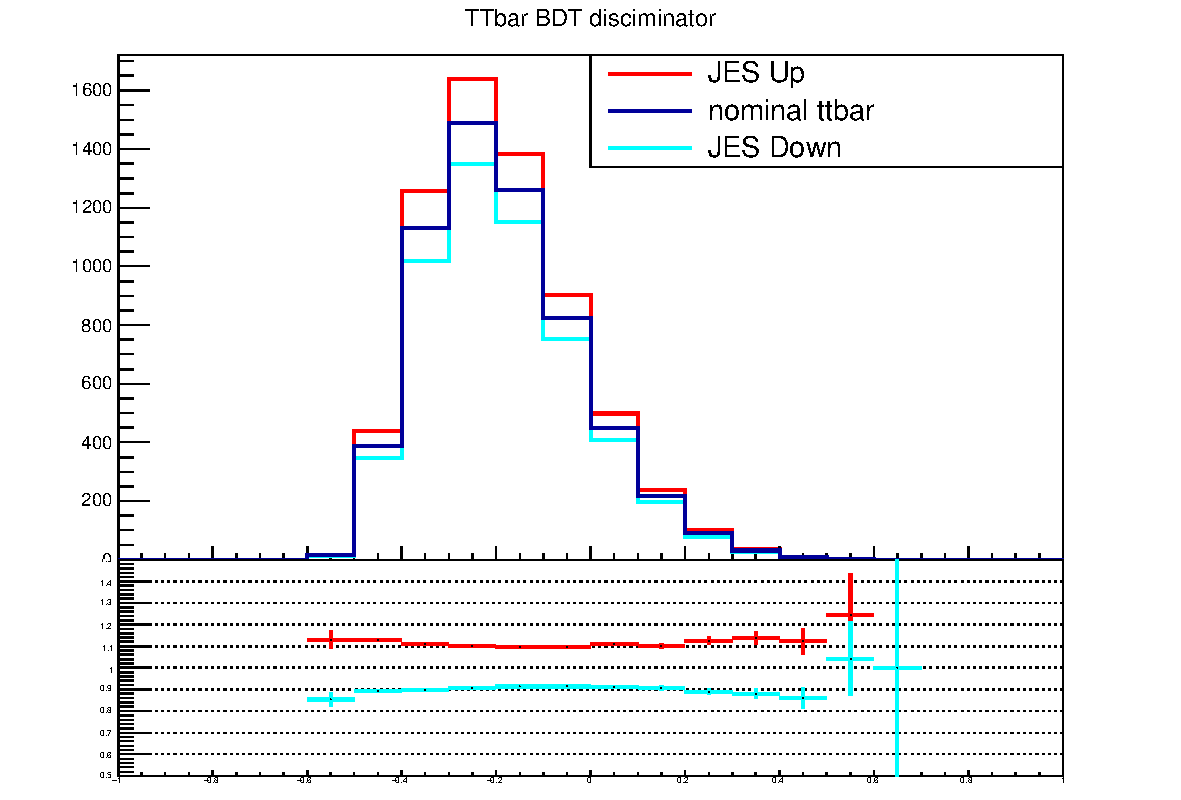
\includegraphics[width=0.48\textwidth]{images/Run2/Sys/JESsystt.pdf}
%     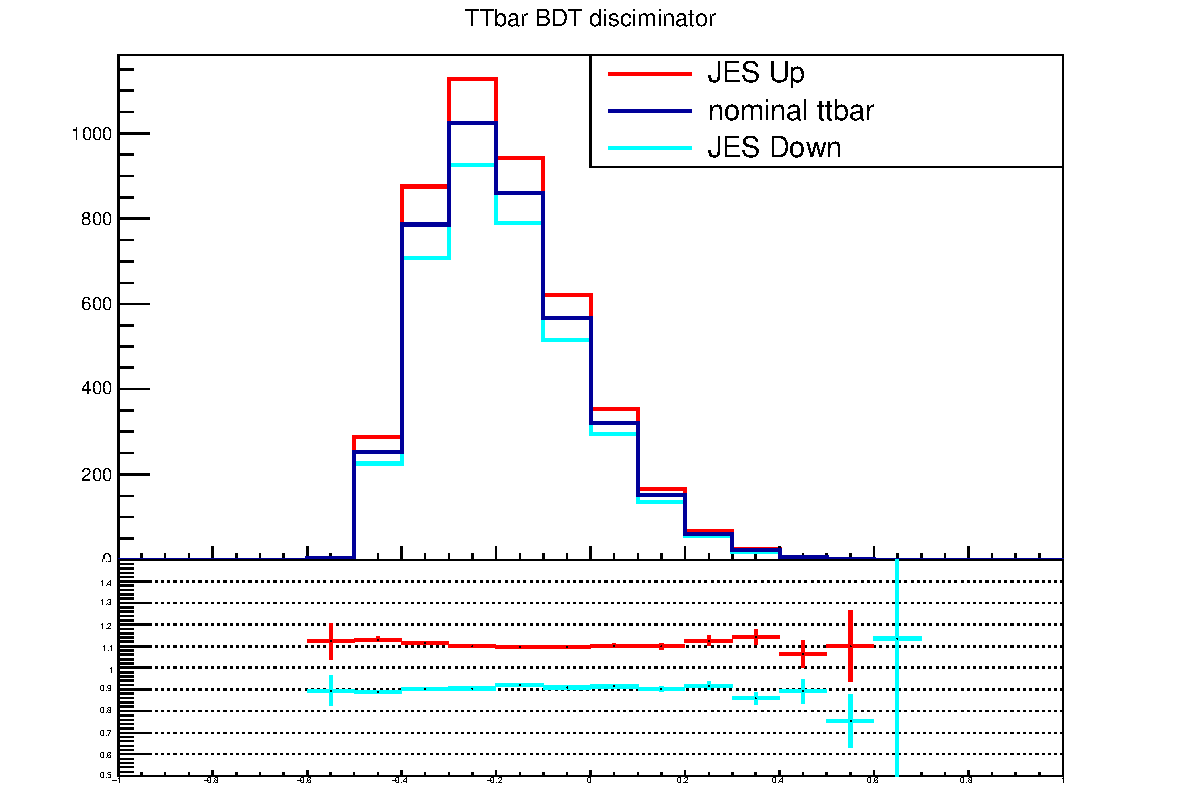
\includegraphics[width=0.48\textwidth]{images/Run2/Sys/JESsystt_e.pdf}     
%     \caption{The BDT shapes for JES systematic in \ttbar for the $\mu$ + jets channel (left) and e + jets channel (right).}
%     \label{fig:SysShapesJEStt}
% \end{figure}

% \begin{figure}[ht!]
%     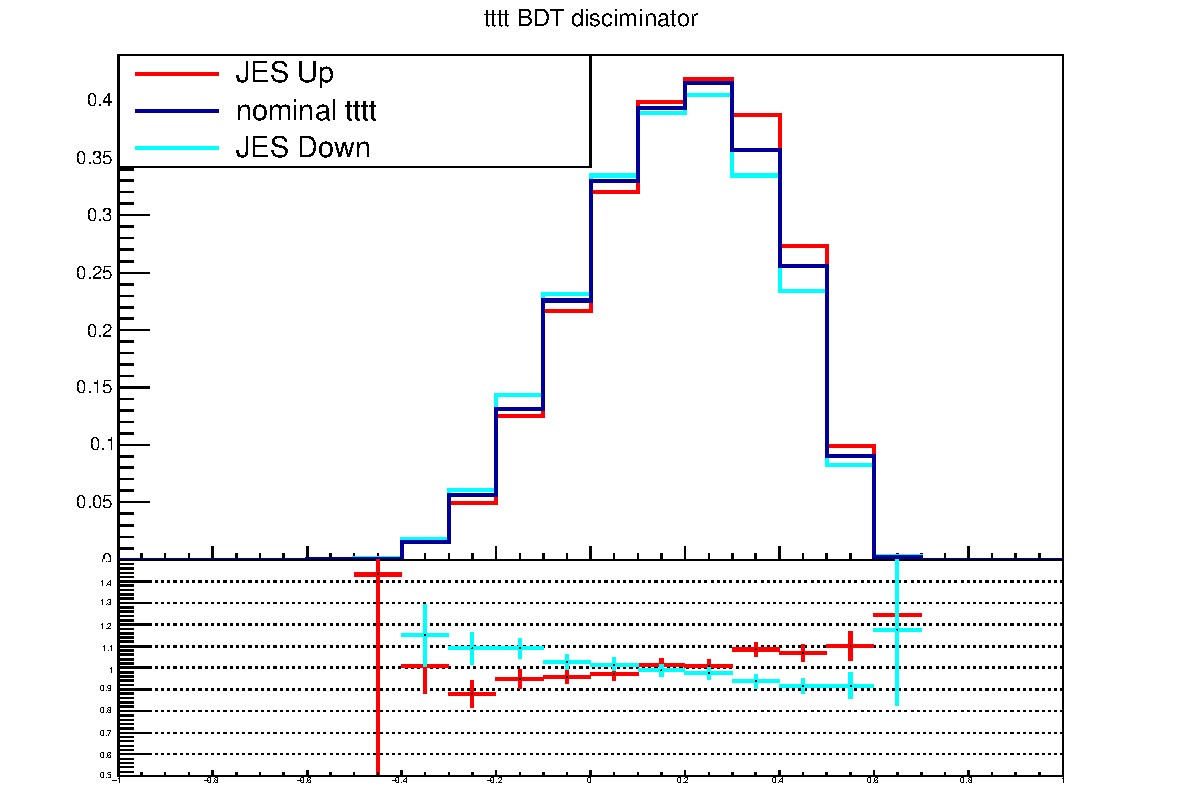
\includegraphics[width=0.48\textwidth]{images/Run2/Sys/JESsystttt.pdf}
%     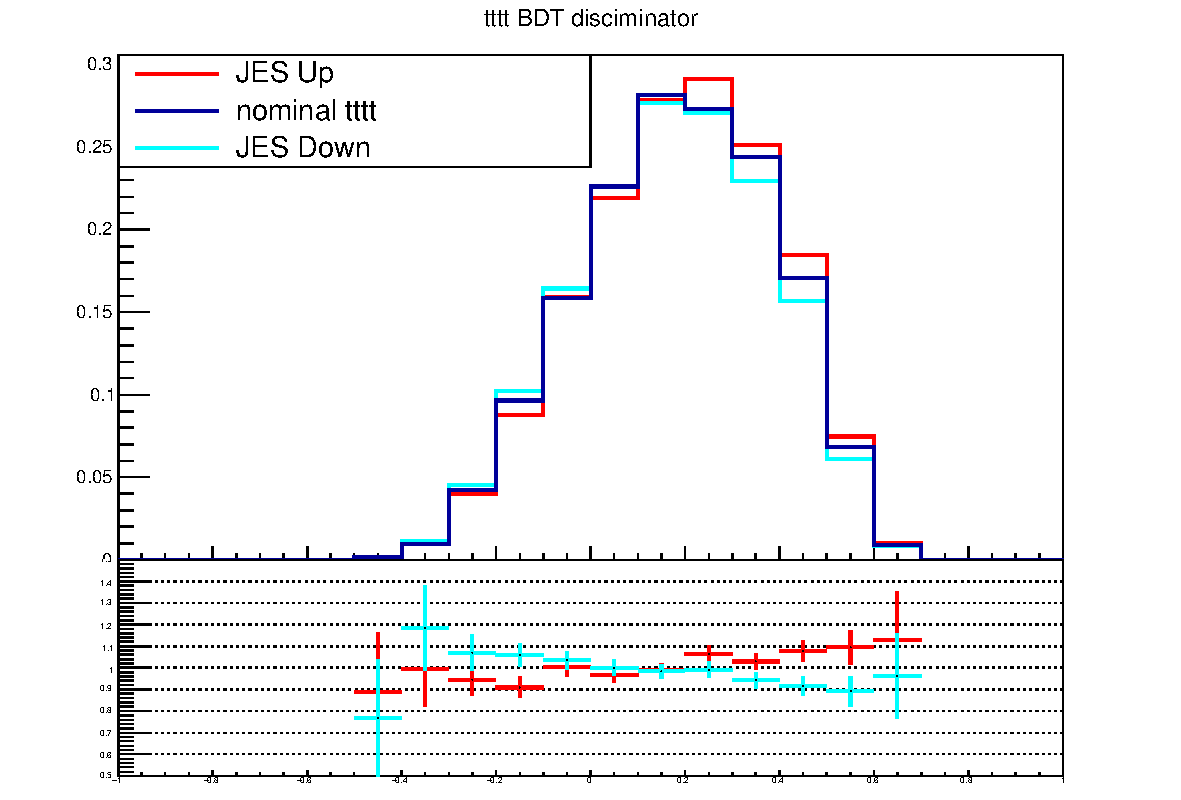
\includegraphics[width=0.48\textwidth]{images/Run2/Sys/JESsystttt_e.pdf}     
%     \caption{The BDT shapes for JES systematic in \tttt for the $\mu$ + jets channel (left) and e + jets channel (right).}
%     \label{fig:SysShapesJEStttt}
% \end{figure}

% \begin{figure}[ht!]
%     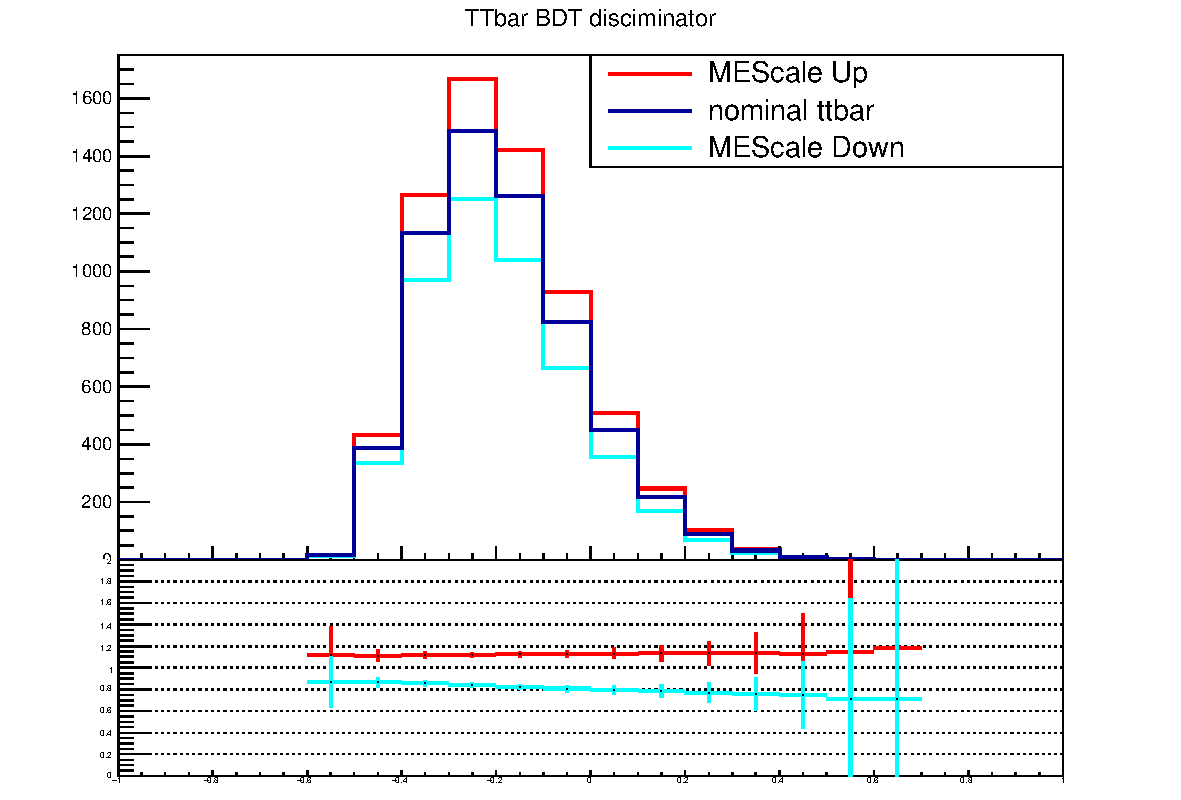
\includegraphics[width=0.48\textwidth]{images/Run2/Sys/MEScalesystt.pdf}
%     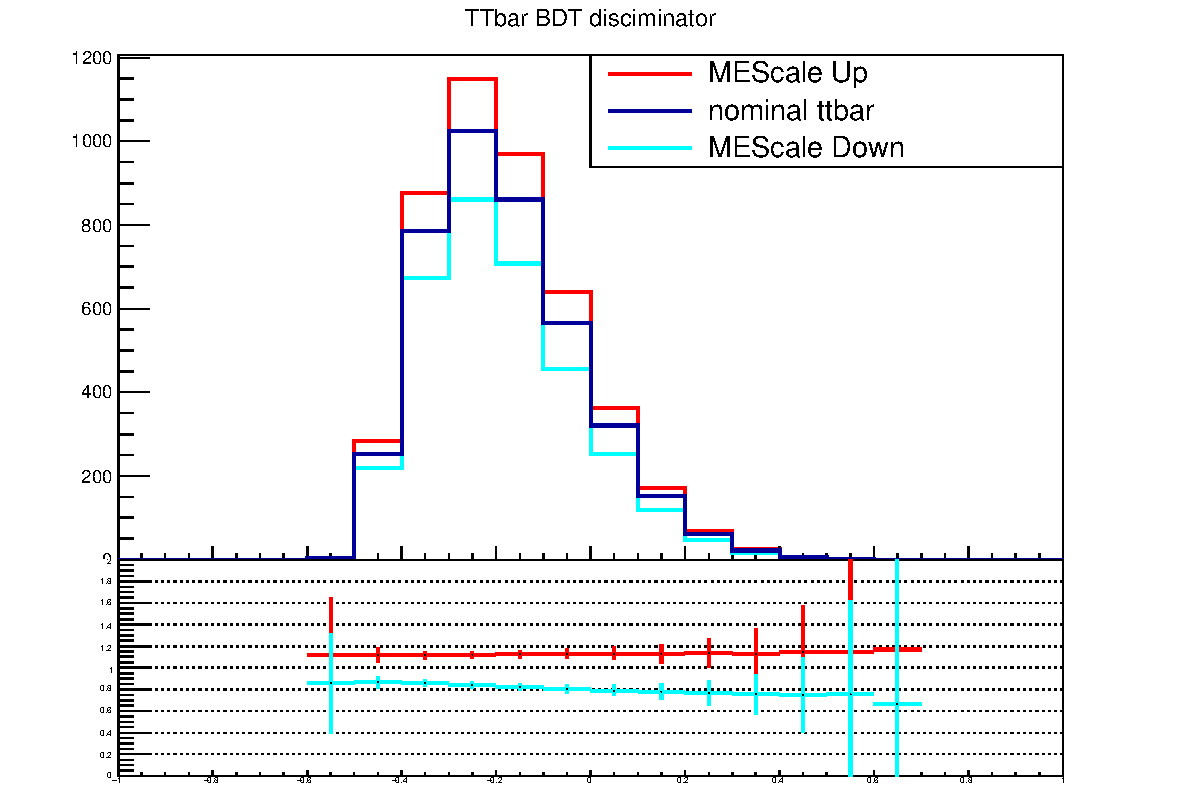
\includegraphics[width=0.48\textwidth]{images/Run2/Sys/MEScalesystt_e.pdf}     
%     \caption{The BDT shapes for ME scale systematic in \ttbar for the $\mu$ + jets channel (left) and e + jets channel (right).}
%     \label{fig:SysShapesMEtt}
% \end{figure}
% \begin{figure}[ht!]
%     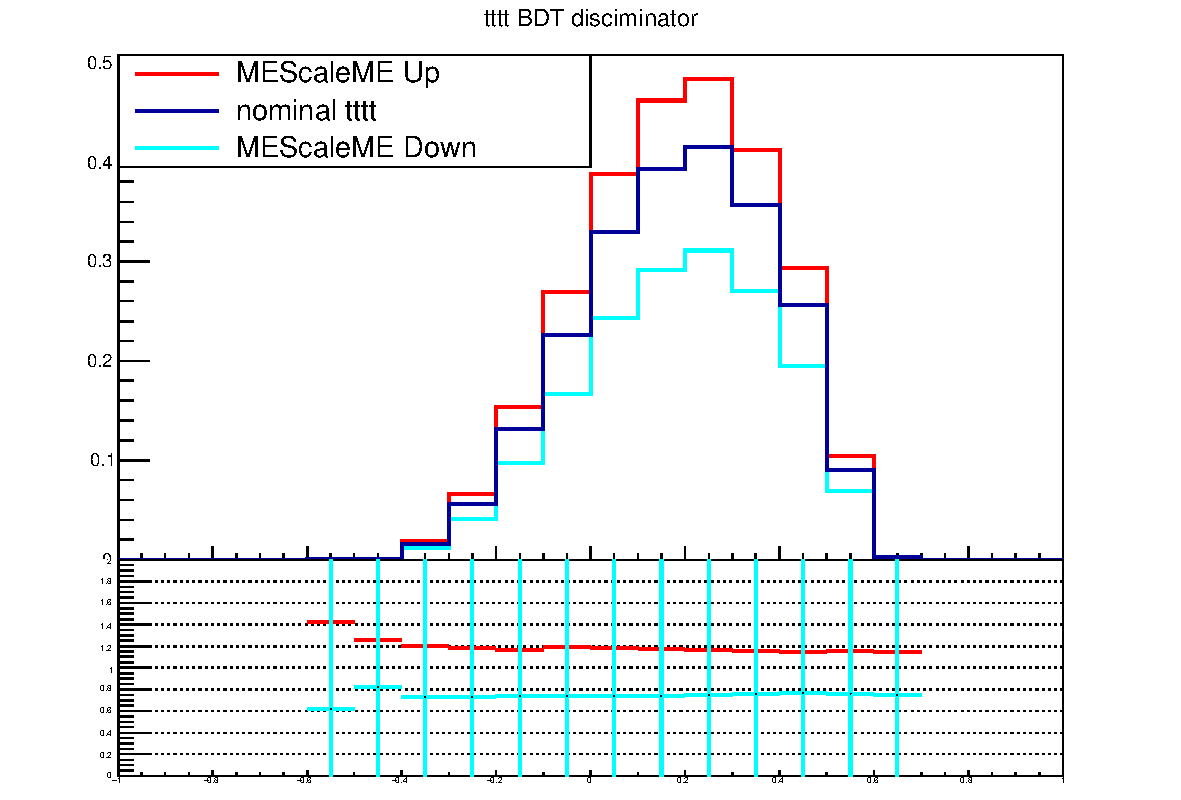
\includegraphics[width=0.48\textwidth]{images/Run2/Sys/MEScalesystttt.pdf}
%     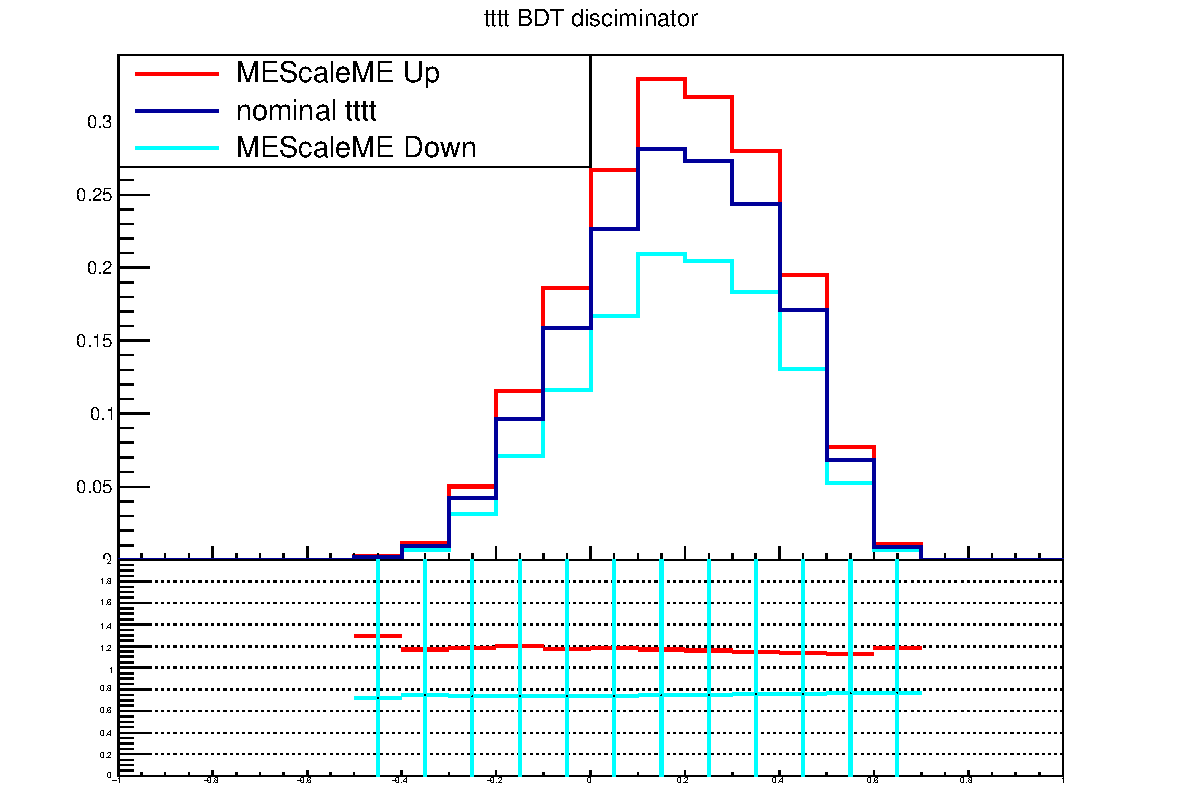
\includegraphics[width=0.48\textwidth]{images/Run2/Sys/MEScalesystttt_e.pdf}     
%     \caption{The BDT shapes for ME scale systematic in \tttt for the $\mu$ + jets channel (left) and e + jets channel (right).}
%     \label{fig:SysShapesMEtttt}
% \end{figure}

% % \begin{figure}[ht!]
% %     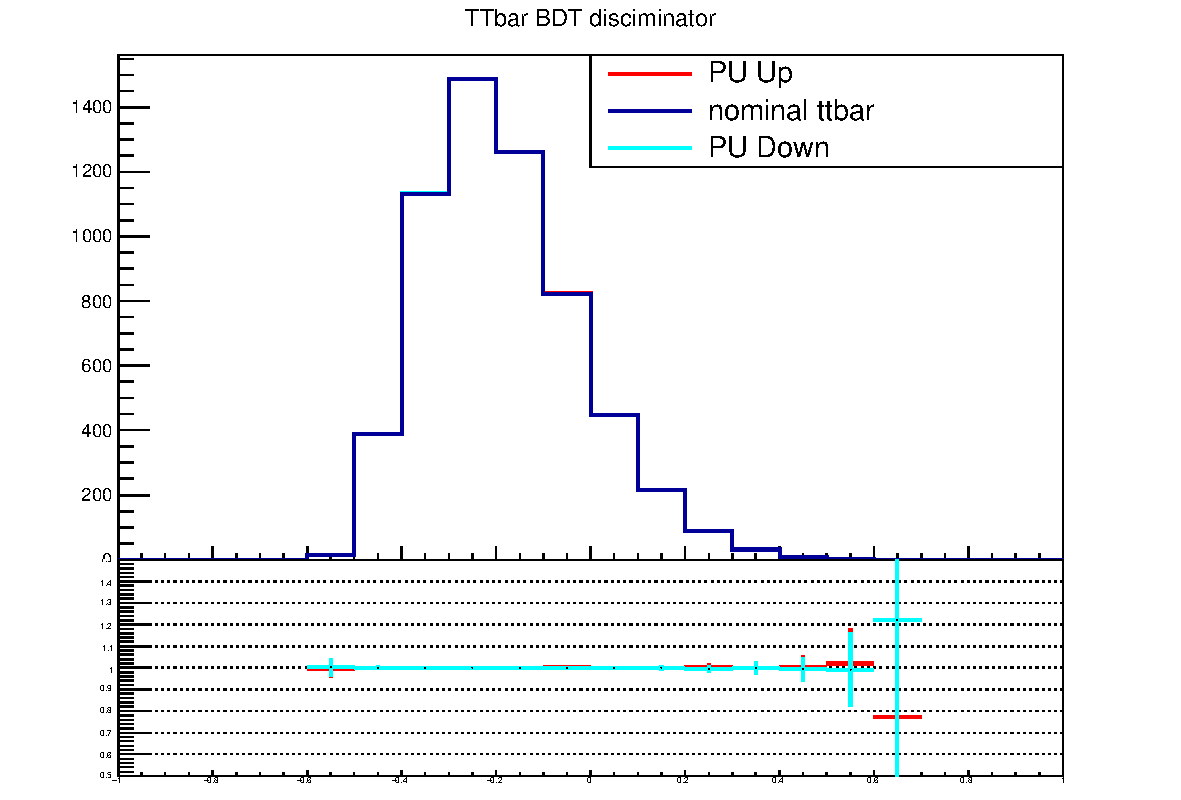
\includegraphics[width=0.48\textwidth]{images/Run2/Sys/PUsystt.pdf} 
% %     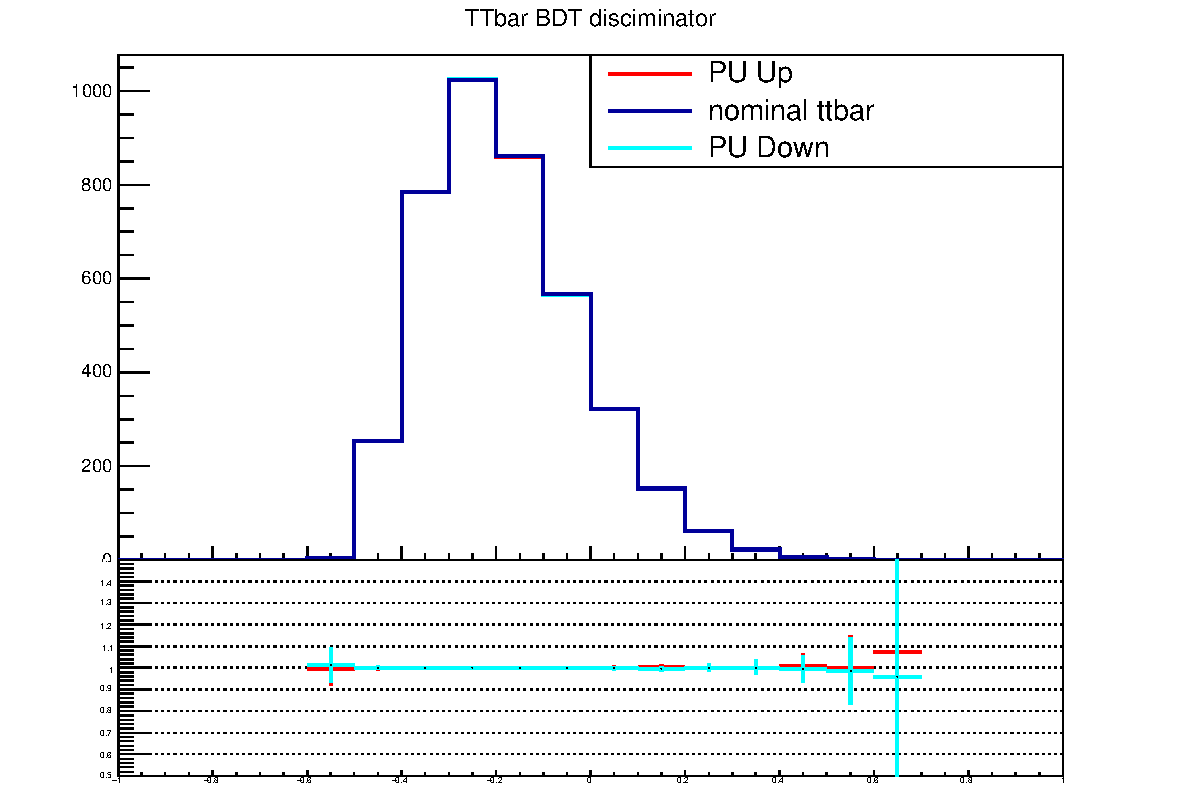
\includegraphics[width=0.48\textwidth]{images/Run2/Sys/PUsystt_e.pdf}     
% %     \caption{The BDT shapes for PU systematic in \ttbar for the $\mu$ + jets channel (left) and e + jets channel (right).}
% %     \label{fig:SysShapesPUtt}
% % \end{figure}

% % \begin{figure}[ht!]
% %     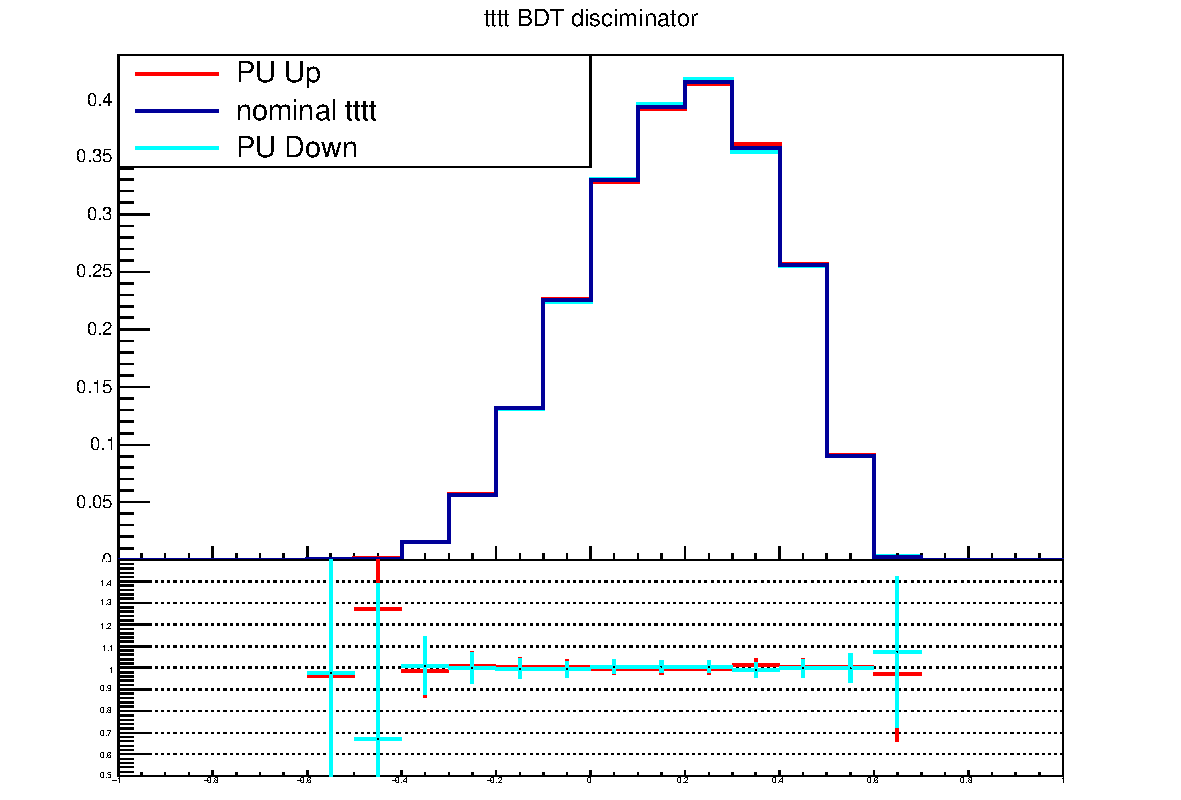
\includegraphics[width=0.48\textwidth]{images/Run2/Sys/PUsystttt.pdf} 
% %     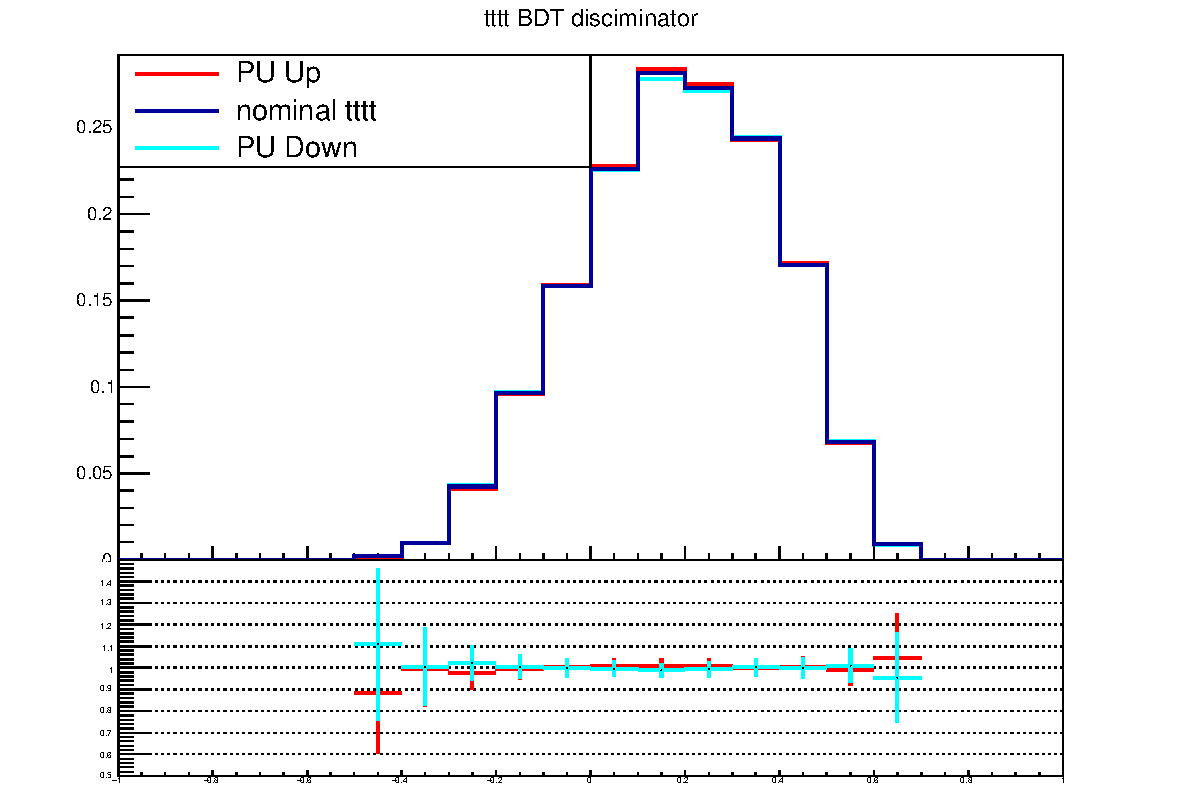
\includegraphics[width=0.48\textwidth]{images/Run2/Sys/PUsystttt_e.pdf}     
% %     \caption{The BDT shapes for PU systematic in \tttt for the $\mu$ + jets channel (left) and e + jets channel (right).}
% %     \label{fig:SysShapesPUtttt}
% % \end{figure}

% % \begin{figure}[ht!]
% %     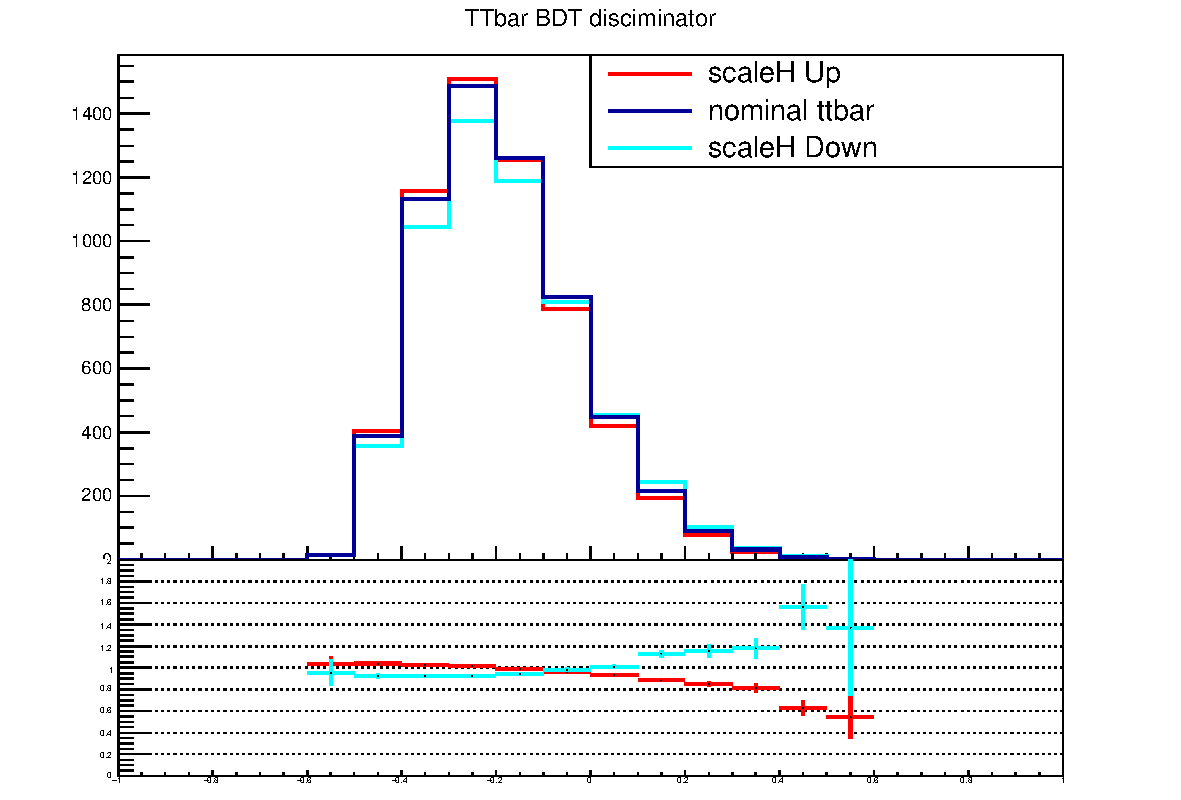
\includegraphics[width=0.48\textwidth]{images/Run2/Sys/ScaleHsystt.pdf}
% %     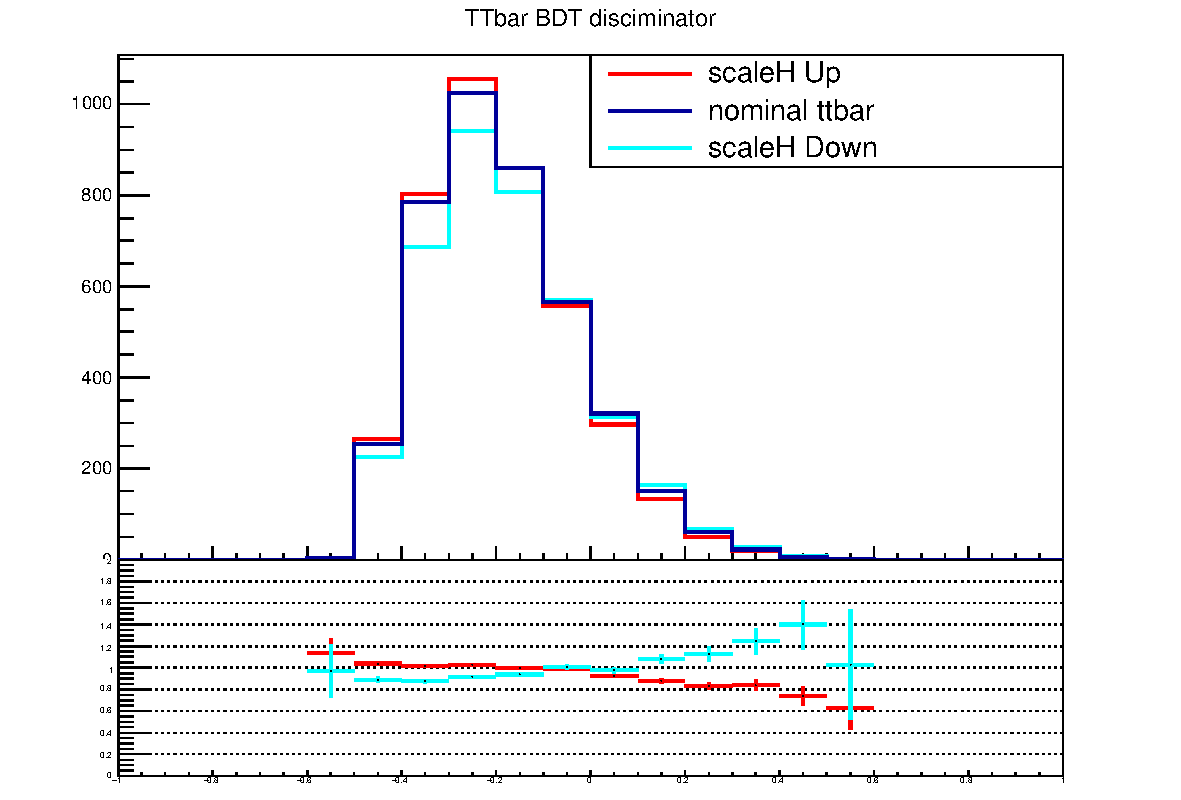
\includegraphics[width=0.48\textwidth]{images/Run2/Sys/ScaleHsystt_e.pdf}     
% %     \caption{The BDT shapes for hadronisation scale systematic in \ttbar for the $\mu$ + jets channel (left) and e + jets channel (right).}
% %     \label{fig:SysShapesScaleHtt}
% % \end{figure}

% \begin{figure}[ht!]
%     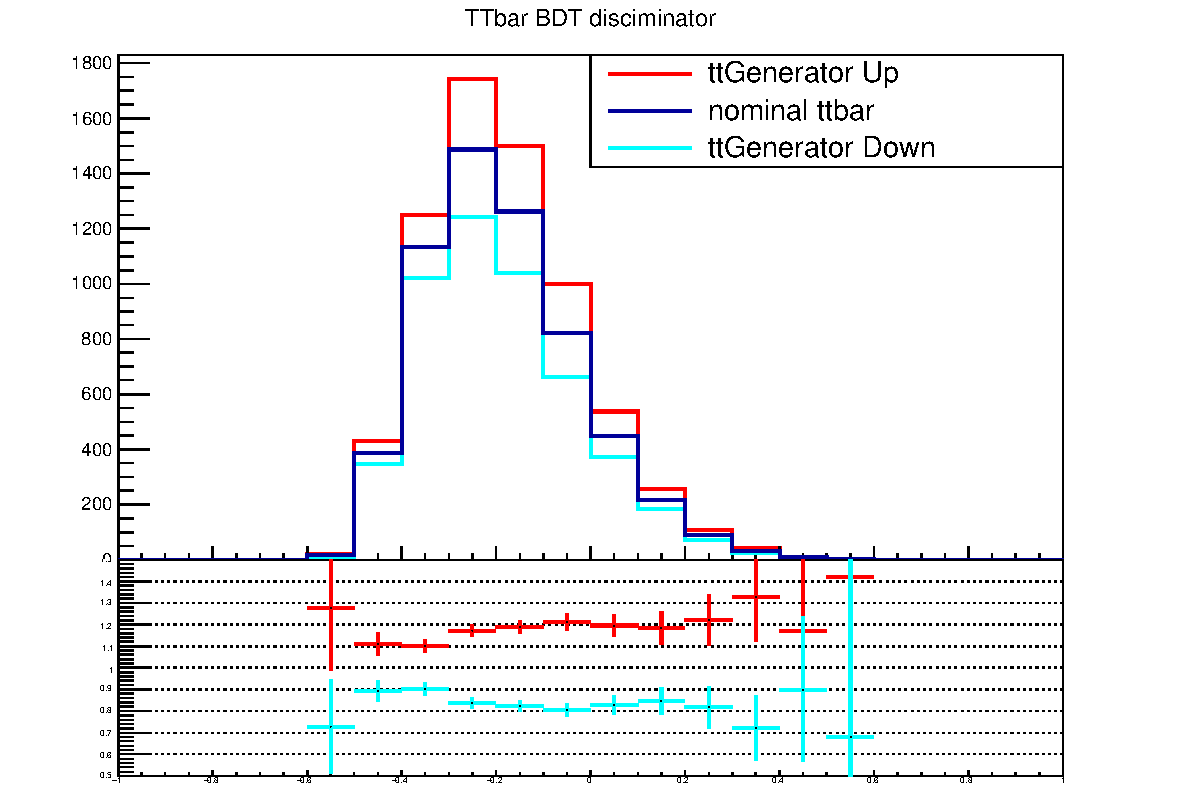
\includegraphics[width=0.48\textwidth]{images/Run2/Sys/ttGeneratorsystt.pdf}
%     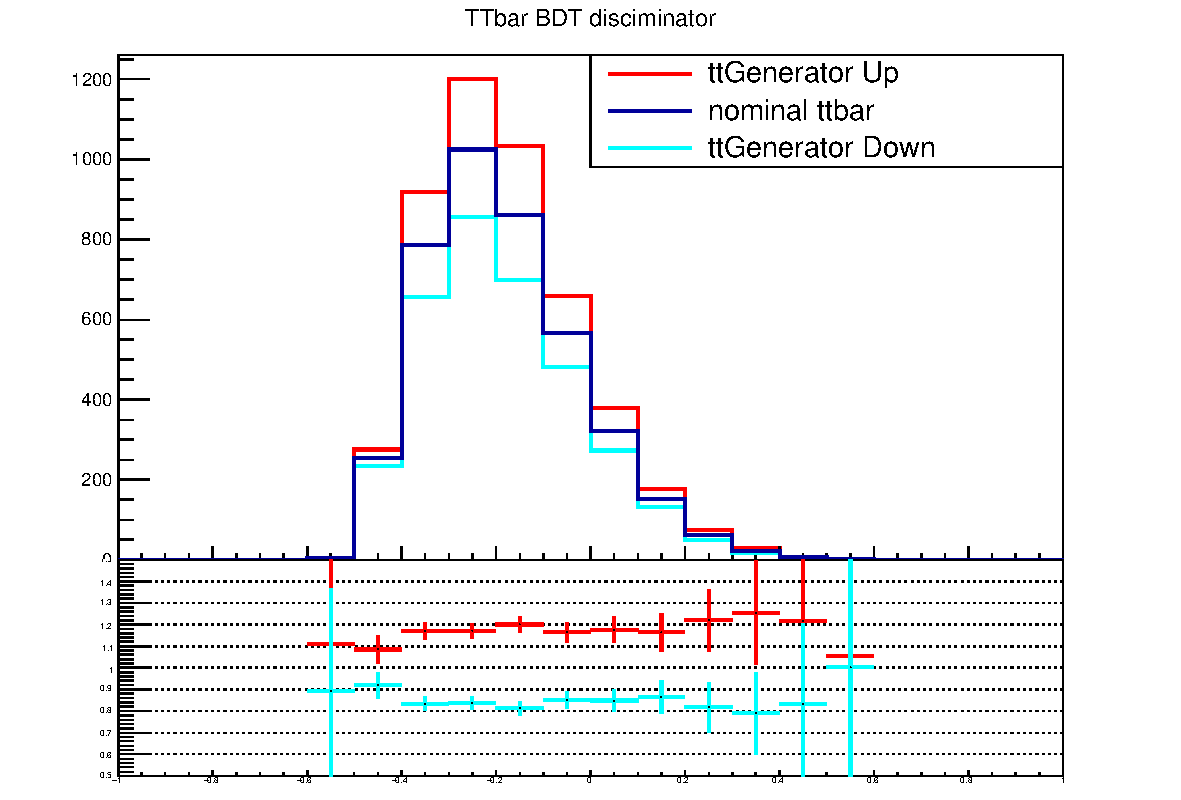
\includegraphics[width=0.48\textwidth]{images/Run2/Sys/ttGeneratorsystt_e.pdf}     
%     \caption{The BDT shapes for ttGenerator choice systematic in \ttbar for the $\mu$ + jets channel (left) and e + jets channel (right).}
%     \label{fig:SysShapesttGen}
% \end{figure}

% \section{Comparison of the Gradient Boost and AdaBoost boosting algorithms within the BDT \label{app:adagrad}}

% For this study, the following three BDTs were trained:
% \begin{enumerate}
% \item \emph{GradNeg} - Gradient boosting taking into account negative weighting information in training and testing
% \item \emph{GradBoost} - Gradient boosting ignoring negative weighting information in training and testing
% \item \emph{AdaBoost} - AdaBoost boosting ignoring negative weighting information in training and testing
% \end{enumerate}
% % It was decided that if we were going to ignore the negative weight information then there was no reason to not include these events in the training sample. Additionally, if one was to ignore the negative weight information then there is no reason to not examine using AdaBoost.  
% % Strategy 1 is referred to as \emph{GradNeg}; strategy 2 as \emph{GradBoost}; and strategy 3 as \emph{AdaBoost}. 
% %
% Each BDT was trained with the same set of input features and using the same sample of events to train and test the BDTs. The expected limits and uncertainties are shown for each strategy in Table~\ref{tab:BDTalgos} for the $\mu$ + jets and e + jets final states. Note that this study was performed at an earlier stage in the analysis so the results to do not correspond to the final expected limit given in Section~\ref{sec:limit13}. The BDT output discriminator distribution was only split into \njets categories of of 6, 7, 8, 9+ jets at this stage rather than \njets and \nMtags categories.
%  % The response of the signal and background samples as well as the ROC curves for the derived classifiers for each strategy can be seen in Figs. \ref{fig:GradNeg} through \ref{fig:AdaBoost}.



% \begin{table}[ht]
% \centering
% \caption{Expected limits using jet categories of 6, 7, 8, 9+ jets for different BDT boosting algorithms.}
% \label{tab:BDTalgos}
% \begin{tabular}{|l|l|l|l|l|}
% \hline
% Algorithm & $\mu$ + jets & uncertainty & e + jets & uncertainty \\ \hline
% GradNeg   & 18.1         & +8.0, -5.3  & 27.6     & +12.9, -8.3 \\ \hline
% GradBoost & 18.7         & +8.3, -5.5  & 28.8     & +12.9, -8.3 \\ \hline
% AdaBoost  & 10.7         & +6.4, -4.0  & 21.6     & +10.9, -7.0 \\ \hline
% \end{tabular}
% \end{table}

% It can be seen from Table~\ref{tab:BDTalgos} that the difference between including negative weight information in the GradNeg strategy and not including it in the GradBoost strategy have a negligible effect on the expected limit within the uncertainties. Using negative weights may slightly optimise the modelling for training but not significantly hence the AdaBoost strategy can be used without negative weights as it has a significant benefit in lowering the expected limit.

% \section{Studies of additional MC samples ~\label{app:altsamples}}


% \subsection{Comparison of alternative \ttbar generators}

% Figure~\ref{fig:MGFXFX} shows that the uncertainty from the \MADGRAPH \aMCATNLO generator is contained within the uncertainty from the \MLM generator, therefore it is conservative to use the \MLM generator as the systematic shape for differences in the BDT distribution due to generator choice.

% \begin{figure}[ht]
% \centering
%     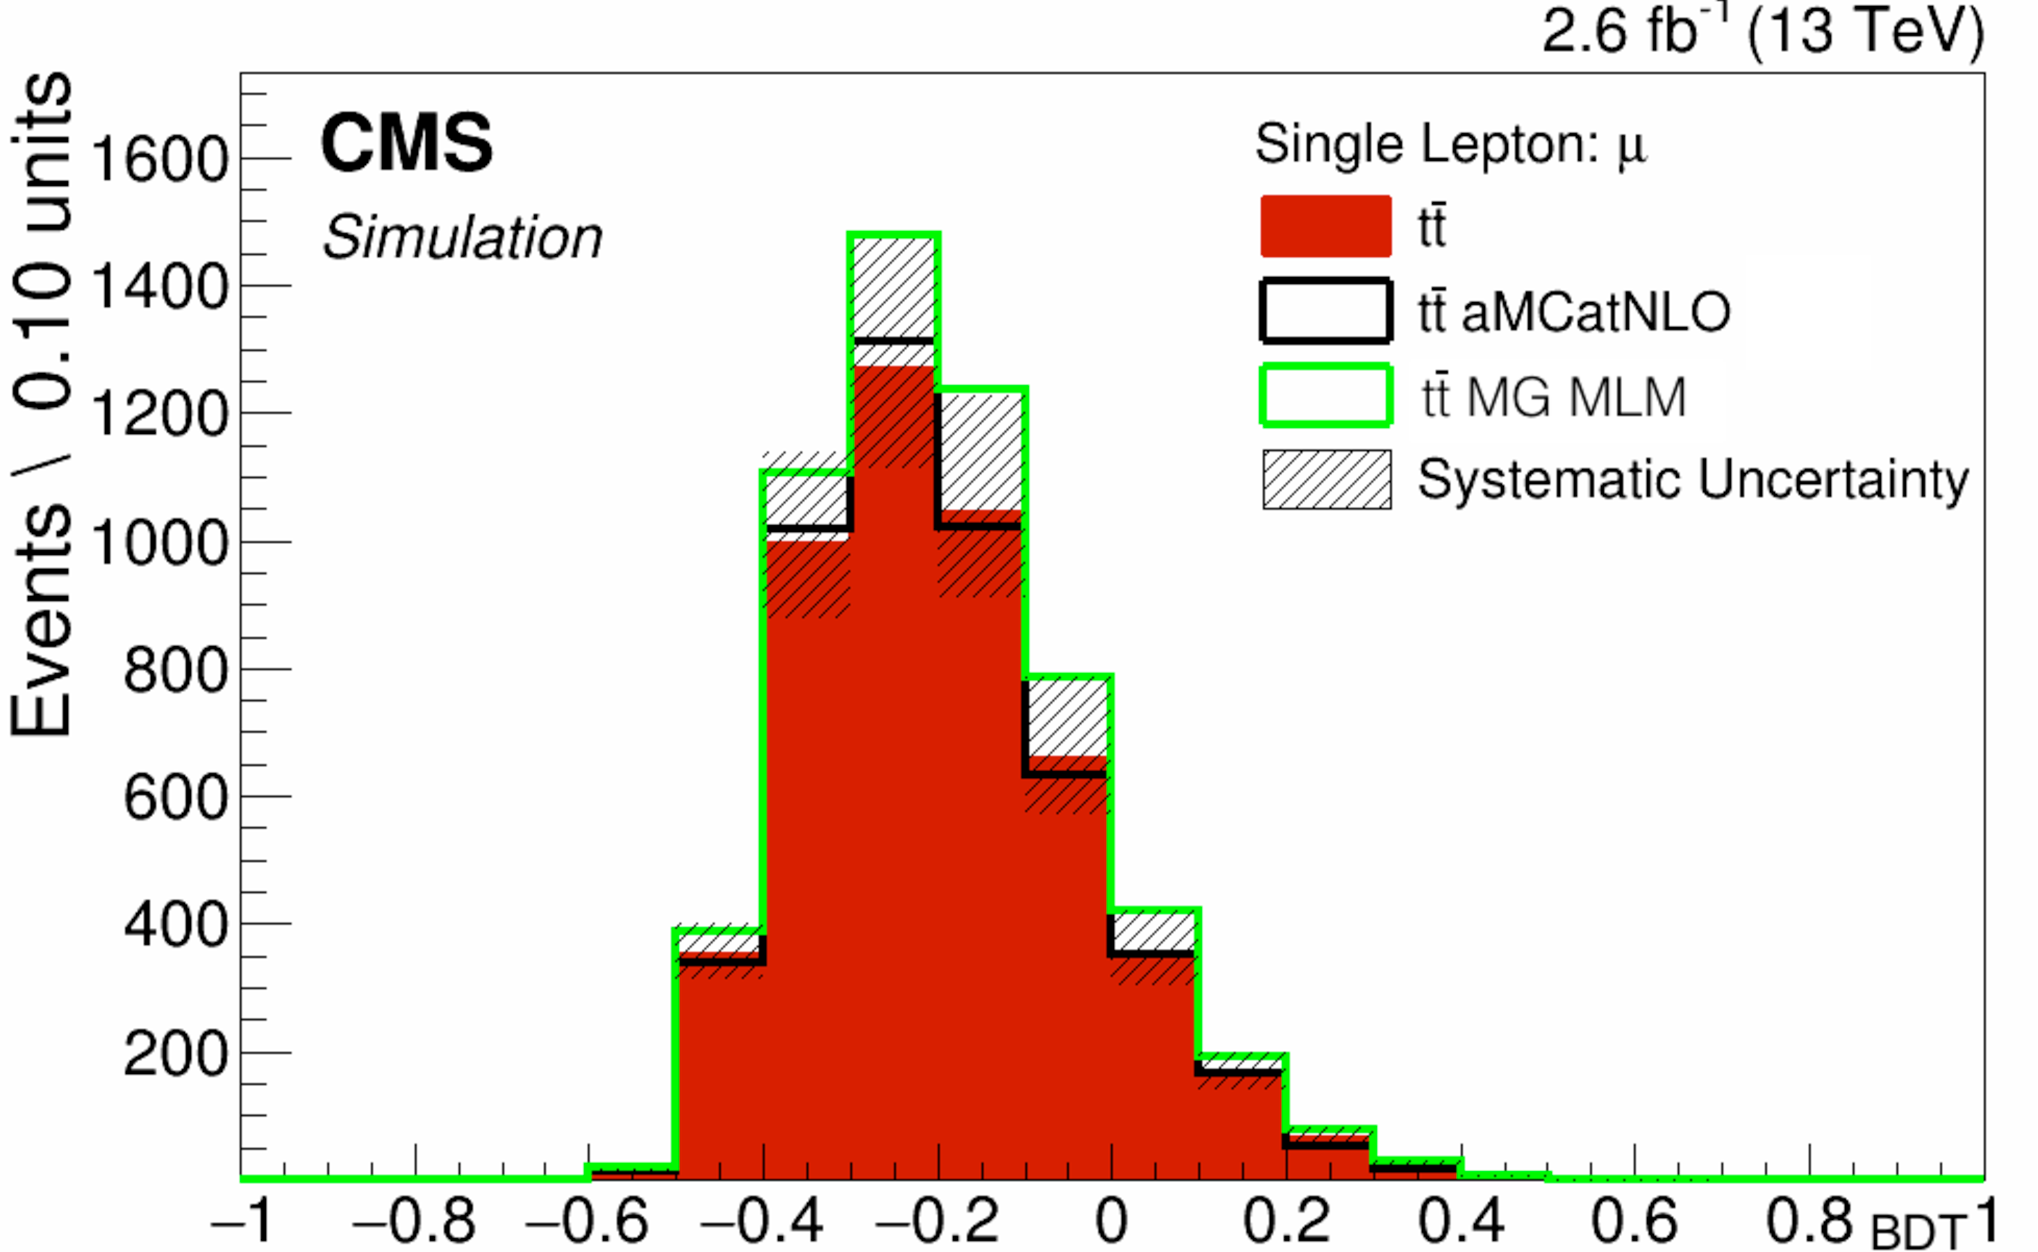
\includegraphics[width=0.7\textwidth]{images/Run2/MG_FXFX.pdf}
%     \caption{Inclusive BDT distribution for \ttbar generators \POWHEG+\PYTHIA, \MLM and \MADGRAPH \aMCATNLO FxFx}
%     \label{fig:MGFXFX}
% \end{figure} 


% \subsection{TTZ, TTW, TTH MC backgrounds~\label{app:TTX}}
% The contributions from \ttbar + B, where B = W, Z or H, were added to the predicted \ttbar yields to give a prediction for the net \ttbar + B background. The event-level BDT discriminant shapes for these contributions closely follow those of the \ttbar contribution and are very different from those predicted for the \tttt signal as a function of both the number of jets and the number of b-tagged jets. The differences are small and they over covered by the \ttbar scale uncertainties. Therefore, no additional systematic uncertainties were considered necessary to cover these backgrounds.


% \begin{figure}[ht]
% \centering
%     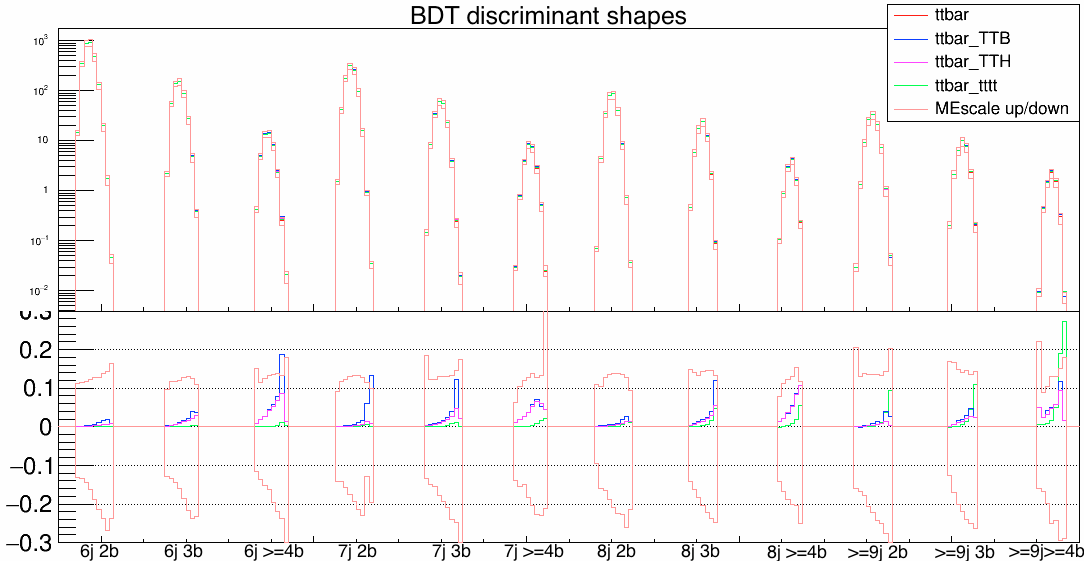
\includegraphics[width=\textwidth]{images/Run2/ttbarShapesLabels.png}
%     \caption{BDT discriminator shapes for all categories, as indicated along the x axis. The ratio plot shows the difference between each distribution and the nominal \ttbar distribution divided by the \ttbar distribution.}
%     \label{fig:TTB}
% \end{figure}


% \section{Combination with OS dilepton channel and SS dilepton channel ~\label{sec:combo13}}

% The sensitivity of the search for standard model four top quark production can be improved by combining with other search channels. An opposite-sign (OS) search was developed in parallel with the single lepton channel study described in this chapter~\cite{CMS-PAS-TOP-16-016}. The analysis selects on events which contain any combination of $\mu^{+}\mu^{-}$, $\mu^{\pm} e^{\mp}$, $e^{+}e^{-}$. It uses the same hadronic top quark reconstruction as in Section~\ref{sec:topContent13} to identify the BDT value for highest-ranked top quark candidate, $BDT_{trijet1}$. This variable is fed into the event-level BDT along with other variables based on the event-topology, event activity and b-jet content. A simultaneous fit was made using the BDT histogram templates described above for the single lepton channel and the BDT histogram templates (which are split only in \njets categories due to statistical limitations) from the dilepton channel. All systematic uncertainties apart from the lepton scale factors were treated as correlated. The results of this fit can be found in table~\ref{tab:limits_combined} in the row labelled \emph{Combined (single lepton and OS dilepton)}. It is clear that the OS dilepton channel alone is not as sensitive as the single lepton channel, which is due in part to it having a smaller branching ratio, however it's combination with the single lepton channel improves the overall sensitivity.\\

% The analysis was then further combined with a search for new physics in events with same-sign (SS) dileptons which places limits on the SM production of four top quarks~\cite{Khachatryan:2016kod}. This search benefits from very low numbers of events from background processes which gives rise to it's good signal sensitivity. The luminosity, JES and PU systematic uncertainties were treated correlated between the SS dilepton channel and the other two channels. The uncertainty in response of the CMS trigger system to events containing dileptons is was also treated as correlated between the two dilepton analyses, whilst all other systematic uncertainties were treated as fully uncorrelated between the SS dilepton analysis and the other two search channels. The combination of all channels is listed in Table~\ref{tab:limits_combined} where it can be seen that this gives a significant improvement in the expected limit compared to any individual channel.

% \clearpage

% \begin{table}[ht!]
% %NOTE: THE VALUES ARE DEFINED IN THE TOP-16-016.tex at the start - modify them there, not here.
%     \caption{Expected and observed 95\% CL upper limits on the SM \tttt production as a multiple of \sigmattttSM and in fb. The values quoted on the expected limits are the $1$ standard deviation uncertainties and include all statistical and systematic uncertainties.}    
%     \centering
%     \small
%     \begin{tabular}{ l | c  |  c | c  | c }
%         Channel  & Expected Limit  & Observed Limit & Expected limit  & Observed Limit \T \B\\  
%          & (x \sigmattttSM) & (x \sigmattttSM) & (fb) & (fb) \T \B \\ \hline 
%                 Single lepton  & $\xsecmusingleptonexp^{\,+\,\xsecmusingleptonup}_{\,-\,\xsecmusingleptondown}$ & $\xsecmusinglepton$ & $\xsecfbsingleptonexp^{\,+\,\xsecfbsingleptonup}_{\,-\,\xsecfbsingleptondown}$ & $\xsecfbsinglepton$   \T \B  \\ 
%                   & & & &  \\

%                 Dilepton  & $\xsecmudileptonexp^{\,+\,\xsecmudileptonup}_{\,-\,\xsecmudileptondown}$ & $\xsecmudilepton$ & $\xsecfbdileptonexp^{\,+\,\xsecfbdileptonup}_{\,-\,\xsecfbdileptondown}$ & $\xsecfbdilepton$ \T \B   \\ 
%                 (opposite sign) & & & &  \\
%             \hline 
%                  Combined (single lep & $\xsecmucomboexp^{\,+\,\xsecmucomboup}_{\,-\,\xsecmucombodown}$ & $\xsecmucombo$  & $\xsecfbcomboexp^{\,+\,\xsecfbcomboup}_{\,-\,\xsecfbcombodown}$ & $\xsecfbcombo$   \T \B  \\
%                 lepton and OS dilepton) & & & &  \\   \hline \hline            
%                 Dilepton & $11.0^{\,+\,6.2}_{\,-\,3.8}$ & $12.9$ & $101^{\,+\,57}_{\,-\,35}$ & $119$   \T \B  \\
%                 (same sign) & & &  & \\ \hline
%                 Combined  & $\xsecmucomboallexp^{\,+\,\xsecmucomboallup}_{\,-\,\xsecmucomboalldown}$ & $\xsecmucomboall$  & $\xsecfbcomboallexp^{\,+\,\xsecfbcomboallup}_{\,-\,\xsecfbcomboalldown}$ & $\xsecfbcomboall$  \T \B   \\
%                 (all channels) & & & &  \\                
%     \end{tabular}
%     \label{tab:limits_combined}
% \end{table}

% \section{Summary and conclusion}
% \label{sec:summary13}

% The SM production of four top quarks at $\sqrt{s} =$~13~TeV has been studied with 2.6~\fbinv of data from the 2015 CMS dataset. In the absence of an excess, limits were placed on the SM cross section, which is 9.2~fb. The single lepton channel was primarily studied in the $\mu$ + jets and e + jets final states. Baseline selection requirements were implemented to suppress backgrounds and select the signal \tttt process. Good agreement was observed between the simulation and data in many variables after corrections were applied to the events. BDTs were employed to reconstruct hadronically decaying top quarks and then to increase the separation of the signal and background processes using several discriminating variables including those formed from the hadronic top quark BDT. Many tests were performed to check the performance of the BDTs, that it didn't suffer from overtraining and was stable with respect to changing hyperparameters. Categorisation of the histograms going into the template fit was optimised to enhance the sensitivity of the analysis and hence reduce the expected limit. The limit set on the SM production of four top quarks is $16.0^{+9.8}_{-5.5}\times \sigmattttSM$ expected and $16.8\times \sigmattttSM$ observed which equates to $147.2^{+90}_{-51}$ expected and 154.6 fb observed.

% \section{Discussion of ATLAS four-top-quark production studies at $\sqrt{s} =$~13~TeV}
% \label{sec:ATLASresult13}
% % \fxnote{Possible comparison with atlas requirements put into our framework}
